%%%%%%%%%%%%%%%%%%%%%%%%%%%%%%%%%%%%%%%%%%%%%%%%%%%%%%
%%
%%           EE474 Pointers in C
%%
%   % combined into notes pack
%
%\documentclass{article}
%\documentclass{seminar}
%
%\newpagestyle{BHstyle}{\sl U. of Washington \hfil EE 474 \hfil \thepage}{Hannaford \hfil \today}
%\pagestyle{headings}
%\slidepagestyle{BHstyle}
%\addtolength\oddsidemargin{3cm}
%\usepackage[T1]{fontenc}
%\usepackage[utf8]{inputenc}
%\usepackage[english]{babel}
%\usepackage{graphicx}
%\usepackage[pdftex,
%    pdftitle={ECE 474: Critical Sections},
%    pdfauthor={Blake Hannaford, University of Washington},
%    pdflang={en-US},
%    pdfsubject={ECE 474 Embedded Microcomputer Systems},
%    pdfkeywords={embedded systems, microcontrollers, ECE 474},
%    hidelinks,
%    unicode]{hyperref}
%\usepackage{listings}
%
%
%\oddsidemargin 0in
%\evensidemargin 0in
%\textwidth 6.5in
%\textheight 8.7in
%\topmargin 0.2in
%
% 
%\linespread{1.0}
%
	%<*>
%\begin{document}
%\begin{slide}
\section*{ Interprocess Communication, Critical Sections}

%%%%** Section 1 
\section{Critical Sections}
	%<*chn>
\subsection*{Introduction}

When processes share a resource (such as blocks of memory
or I/O devices) we have to think very carefully about coordinated
use of the resource.  Humans find this relatively easy (in
simple cases of course) but time-shared processes in a computer
are a different story.

We will illustrate these issues with the producer-consumer
problem.  We will simulate the operation of the tasks in-class
using people in place of the CPU.  We will use plastic buttons
for data items, and the chalkboard will represent RAM (for
counters flags etc).

\subparagraph{Producer} A task which generates blocks of data.

\subparagraph{Consumer} A task which does something with the data
blocks and discards them or passes them to another consumer.

	%<*>

%\end{slide}
%\begin{slide}


%%%%** Section 1.1
\subsection{Producer-Consumer Example}

\subparagraph{Producer} A task which generates blocks of data.

\subparagraph{Consumer} A task which does something with the data
blocks and discards them or passes them to another consumer.

\subparagraph{Human Example}   An in-class exercise to illuminate
the problem.

%\end{slide}
%\begin{slide}


%%%%** Section 1.1.1 
\subsubsection{Human instructions: Producer }
\begin{verbatim}
If there is room
   add item to shared buffers
else
   wait;
\end{verbatim}


%%%%** Section 1.1.2 
\subsubsection{Human instructions: Consumer }
\begin{verbatim}
If an item available
   take item from shared buffers
else
   wait;
\end{verbatim}


%\end{slide}
%\begin{slide}


%%%%** Section 1.2
\subsection{Pseudo Code Producer-Consumer}
%%%%** Section 1.2.1 
\subsubsection{ Globals }
\begin{verbatim}
/* example.h   */
#define BSIZE = 5
typedef item {plastic button(!)};
struct item ConsIt,NextIt, buffer[BSIZE];
int in=0, out=0, count=0;
\end{verbatim}

%\end{slide}
%\begin{slide}


\begin{tabular}{p{2in}p{2in}}

\begin{verbatim}
##### PRODUCER ######
#include example.h
while(1)
   {
   while(count >= BSIZE);
   count++;
   NextIt = {produce an item};
   buffer[in] = NextIt;
   in++;
   if(in >= BSIZE) in = 0;
   }
\end{verbatim}

&

\begin{verbatim}
##### CONSUMER #####
#include example.h
while(1)
   {
   while(count==0); //"spinlock"
   count--;
   ConsIt = buffer[out];
   out++;
   if(out >= BSIZE) out = 0;
   Take(ConsIt);   /*Consume the item*/
   }
\end{verbatim}
\end{tabular}

%\end{slide}
%\begin{slide}

%%%%** Section 1.3
\subsection{Procedures}

\begin{itemize}
        \item 3 volunteers:
        \begin{itemize}
                \item Producer
                \item Consumer
                \item Memory Device (writes on chalkboard)
        \end{itemize}
        \item Condition 1: Two Cooperating Humans
                (Human Instructions)
        \item Condition 2: Two Humans ``executing''
                pseudocode.
        \item Condition 3: One Human Multitasking based
                on pseudocode. (pre-emptive context switches)
        \item Variations:  try two producers or two consumers
        or both.

\end{itemize}

%
%\paragraph{Cases which cause synchronization errors:}
%
%\begin{itemize}
%        \item count == 0, start producer, {\bf interrupt} after count++.
%        Consumer thinks there is an item.
%        \item count == 5, start consumer, {\bf int} after count--.
%        Producer thinks space is available.
%        \item Two Producers: count == 4, {\bf int } producer 1  before count++.
%        Producer 2 produces a token, returns.   Producer 1 now tries to
%        overflow.
%        \item Two Consumers:  count == 1, {\bf int} consumer 1 before count--.
%        Consumer 2 takes token, returns.  Consumer 1 now tries to take when
%        nothing available.
%\end{itemize}
	%<*>


%\end{slide}
%\begin{slide}

%%%%** Section 2 
\section{Intertask Communication and Data Sharing}

%%%%** Section 2.1
\subsection{Passing Data I: Shared Memory}

\begin{itemize}
        \item Global Variables
        \item Shared Buffer
        \item Ring Buffer
        \item FIFO
\end{itemize}


%\end{slide}
%\begin{slide}
%%%%** Section 2.1.1 
\subsubsection{Shared Buffer(s)}
Producer fills a buffer

Signals Consumer

Consumer clears buffer

Multiple buffers:  Producer fills buffer A
{\it while} Consumer clears buffer B.

switch pointers A and B

This scheme is called "double buffering".  Allows producer and
consumer to work simultaneously.

%\end{slide}
%\begin{slide}
%%%%** Section 2.1.2 
\subsubsection{Ring Buffer / FIFO}

One buffer.    Two Pointers *in, *out.
 Also called ``FIFO'' --- First-In-First-Out	%<ch>

Producer:
\begin{verbatim}
   while(in != out) {
      buffer[in++] = {new data item}
      if(in >= BUFFER_SIZE) in = BUFFER;
      }
   print "BUFFER OVERFLOW!!!!" ; halt;
\end{verbatim}
Consumer:
\begin{verbatim}
   while(out != in ) {
      data = buffer[out++];
      if(out >= BUFFER_END) out = BUFFER;
      }
   print "BUFFER UNDERFLOW!!!!" ; halt;
\end{verbatim}



%\end{slide}
%\begin{slide}
%%%%** Section 2.1.3 
\subsubsection{LIFO}
``Last-In-First-Out''

A stack

One buffer.  One pointer *iop

Producer:
\begin{verbatim}
   while(iop <= BUFFER_END) {
      buffer[iop++] = {new data item}
      }
   print "LIFO OVERFLOW!!!!" ; halt;
\end{verbatim}
Consumer:

\begin{verbatim}
   while(iop != BUFFER ) {
      data = buffer[--iop];
      }
   print "LIFO UNDERFLOW!!!!" ; halt;
\end{verbatim}


%\end{slide}
%\begin{slide}
%%%%** Section 2.2
\subsection{Passing Data II: Message Passing}
Problem with shared memory approaches is that processes are not protected from
each others bugs.

OS can isolate processes better by supporting messages.

Two types:
\begin{itemize}
	\item Message Passing
	\item Mailbox
\end{itemize}

%\end{slide}
%\begin{slide}
Example:
\begin{verbatim}
/*  Process 1
 */
while(1) {
   compute & produce data;
   OS_send_message(Proc_ID);
   }
\end{verbatim}

%\end{slide}
%\begin{slide}
%%%%** Section 2.3
\subsection{Passing Data III: Mailboxes}


Example:
\begin{verbatim}
/*  Process 1
 */

mailboxname="mailbox1_2";
mailboxstatus = OS_mailbox_setup(mailboxname);
if(mailboxstatus != MB_SUCCESS)
       error_exit("Couldn't setup mailbox");
while(1) {
   compute & produce data;
   OS_post_message(mailboxname);
   }
\end{verbatim}

%\end{slide}
%\begin{slide}
\begin{verbatim}
/*  Process 2
 */
mailboxname="mailbox1_2";
// assume mailbox has been setup by Proc 1
while(1) {
   OS_pend_message(mailboxname);
   consume data;
   }
\end{verbatim}

%\end{slide}
%\begin{slide}
OS message calls invoke the scheduler.

Sender is set to {\tt WAITING} until receiver gets the message.

Receiver is set to {\tt WAITING} until mailbox contains a message.

%\end{slide}
%\begin{slide}
%%%%** Section 2.4
\subsection{Networked and Multiprocessor Environments}
If OS supports it, can communicate across networks and between processors.

Message passing:    {\tt Proc\_ID} $\to$ {\tt host:Proc\_ID}

Mailboxes:     {\tt mailboxname} $\to$ {\tt "host:mailbox" }



%\end{slide}
%\begin{slide}

%%%%** Section 3 
\section{Concurency Problem Statement}

Fundamental Problem: make sure only one task accesses a resource
during ``Critical Section".

{\it Critical Section: } a short segment of code which must be done
as a unit (also called ``atomic" operation).

Above example: testing buffer counter and taking/putting token
must be done together without interruption.


%\end{slide}
%\begin{slide}

%%%%** Section 3.1
\subsection{Remedies}

%%%%** Section 3.1.1 
\subsubsection{ Mask Interrupts}

Make an OS call, or manipulate bits in interrupt controller
to prevent any ISRs from running during Critical Section.

Example:
\begin{verbatim}
...
OS_INT_MASK();  // block all interrupts
 if(data_avail_flag) {
        // if ISR occurs here ---> Trouble!!
          process(buffer);
          data_avail_flag = FALSE;
          buffer_avail_flag = TRUE;
          }
OS_INT_ENABLE();
...
\end{verbatim}

This prevents

1) pre-emption by scheduler which would
start another task.

2) An ISR which may mess with
buffers/ptrs.

%\end{slide}
%\begin{slide}
\subsection*{Int Masking: pro/con}

\noindent
{\bf Pros:}

  Fast

\noindent
{\bf Cons:}

Too greedy:  blocks all I/O devices and other tasks whether
they use the key resource or not!


%\end{slide}
%\begin{slide}
%%%%** Section 3.1.2 
\subsubsection{Test and Set}

A Machine Language Instruction (first on IBM 360)

\begin{verbatim}

# assembler:
        TSR     R,FailAddr   # jump to FailAddr if R ne 0
# explanation:
        if(R==0) R = 1 ;
        else jump FailAddr ;
\end{verbatim}

{\tt TSR } is a single instruction and cannot be interrupted.

Example (pseudo assembler code):
\begin{verbatim}
x = 0;
while(1) {
Wait:   TSR  X, Wait ;  // wait for x==0
        //
        // Critical Section Code
        //
        MOVI    X, 0 //  Release Flag X
        ...
        }
\end{verbatim}


%\end{slide}
%\begin{slide}
\subsection*{Test and Set Pros and Cons}

{\bf Pros:}

 Extremely fast

 Can be specialized for many resources without
 blocking unnecessarily.

{\bf Cons:}

  Very low-level.   Who decides what ``{\tt X}" is
  for each resource?

  Only allows one user per resource. What if resource
  permits {\tt N} users?

%\end{slide}
%\begin{slide}

%%%%** Section 3.2
\subsection{Semaphores}

Term Origin: Flags used in signaling.

An OS facility which guarantees exclusive access.

Three OS Calls:

\begin{verbatim}
semaphore os_get_semaphore(int N);
    // establish a new semaphore
    // initialize to N

void os_pend(semaphore S);
    // wait for resource protected by S

void os_post(semaphore S);
    // free up resource protected by S

\end{verbatim}

%\end{slide}
%\begin{slide}

%%%%** Section 3.2.1 
\subsubsection{Semaphores: Pend and Post}

Identify the critical section in your code.

"protect" it with {\tt Pend(S)} and {\tt Post(S)}:
\begin{verbatim}

...
pend(S);

  critical section code

post(S)
\end{verbatim}


%\end{slide}
%\begin{slide}

%%%%** Section 3.2.2 
\subsubsection{Implementing Pend and Post inside a kernel}
{\bf Notes:   }

S is typically a small integer.

S==0 $\to$ wait,  S $\geq$ 1 $\to$ go


Pend(S):
\begin{enumerate}
  \item disable interrupts
  \item {\tt if (S$>$0) \{ S--; Enable Interrupts; return\}}
  \item else {\tt \{Enable Interrupts; set task to `WAIT'; store S in TCB.sem;  start scheduler\}}
\end{enumerate}

Post(S):
\begin{enumerate}
  \item S++
  \item start scheduler
\end{enumerate}

%\end{slide}
%\begin{slide}


%%%%** Section 3.2.3 
\subsubsection{Critical Section Summary}

The {\bf Contention Problem} can occur under two conditions:
\begin{enumerate}
	\item There is preemption due to interrupts.
        \item Two or more processes share a single resource.
\end{enumerate}
A {\bf Critical Section} is the part of code which, if interrupted, could cause a bug in sharing a resource between
two processes.

Example:   Increment a counter and then put data in buffer.

{\bf Semaphores} can be used to protect a critical section.

\begin{enumerate}
	\item One semaphore, S,  is established for each shared resource.
        \item pend(S) operation is used at start of critical section.
        \item post(S) operation is used at end of critical section.
\end{enumerate}

Pend means ``wait" (i.e. ``patent {\it pend}ing").

Scheduler makes sure that tasks waiting for a resourse (i.e. pending a semaphore)
are set to ``WAITING" and that other tasks can run instead.




%\end{slide}
%\begin{slide}

\subsubsection*{Semaphores: Pros and Cons}
{\bf Pros:}

Specialized, one semaphore per resource, no
unnecessary blocking.

Widely used standard.

Low to medium implementation overhead in O/S.

{\bf Cons:}

Can cause {\it Piority Inversion}



%\end{slide}
%\begin{slide}

%%%%** Section 3.2.4 
\subsubsection{Priority Inversion}

Consider the following scenario.

(low numbers = high priority)
\begin{verbatim}
Task A    Priority  5
Task B    Priority 10
Task C    Priority 15
\end{verbatim}

	%<*chn>
Suppose tasks A, and C, both  want to use a buffer protected by semaphore {\tt S},
but task B does not.
%
%Task A, C $\to$ Buffer $\to$ {\tt semaphore S}
	%<*>
\begin{enumerate}
        \item Task C is running and uses {\tt OS\_pend(S)} to
        get the buffer.  OS grants the buffer to C and C computes
         slowly on buffer.
        \item Task A starts.  Task A also requests buffer by {\tt OS\_pend(S)}.
          It has to wait for C to finish with {\tt S}.
        \item With Task A still waiting, Task B starts.
        \item C is pre-empted by an interrupt.
        \item Scheduler runs B.  Although B does not even want the
        buffer (semaphore S),   it has higher
        priority than A,  and blocks A ...
        
        \item C is effectively blocked by lower priority task B. \\
        (C is waiting for A to release semaphore({\tt S}).
\end{enumerate}


%\end{slide}
%\begin{slide}

%%%%** Section 3.2.5 
\subsubsection{Priority Inversion Remedies}

 \begin{itemize}
        \item Priority Inheritance.  O/S has to check each
        semaphore {\tt pend}.

        If a higher priority process is blocked by a {\tt pend},
        process {\it having the resource} temporarily gets priority
        equal to the {\it blocked} process.

        \item Priority Ceiling Protocol.

        When getting a resource, process temporarily gets priority
        equal to highest process sharing that resource.

\end{itemize}


%\end{slide}
%\begin{slide}

\subsection*{Just google:}
\hspace{0.5in}``priority inversion mars JPL"

\begin{center}
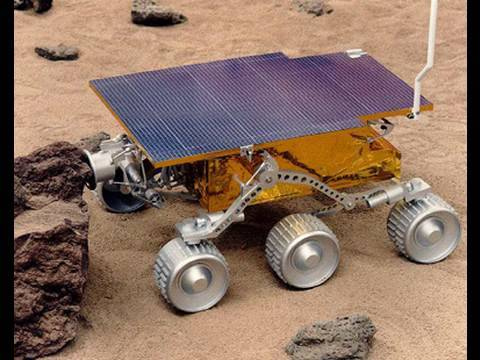
\includegraphics[width=2in]{misc_figs/pathfinder.png}
\end{center}
 

%\end{slide}

%\end{document}























